\chapter{Introduction}

%TODO: add references
\pagenumbering{arabic}
Particle physics is an established branch of physics with a rich history in theory and experiments ever since the beginning of the 20th century. So far the experimental and theoretical research have shown us hand in hand that the universe consists of particles and force carriers. Particles of matter, or elementary particles, are divided into two groups, quarks and leptons. The quarks that we know today are called $u$ (up), $d$ (down), $s$ (strange), $c$ (charm), $b$ (bottom) and $t$ (top). Leptons are  further split into two groups; charged leptons $e$ (electron), $\mu$ (muon), $\tau$ (tau lepton) and their corresponding neutrinos $\nu_e$ (electron neutrino), $\nu_\mu$ (muon neutrino), $\nu_\tau$ (tau neutrino). Particles of force are known as gauge bosons and they are $\gamma$ (photon), $g$ (gluons), $W^\pm$ (charged weak bosons) and $Z^0$ (neutral weak boson). Theory also predicted the recently discovered Higgs boson ($H$), which is responsible for the mass of all particles. Some of the particles above also have a mirrored version of themselves, called antiparticles, which exhibit somewhat different properties as their un-mirrored versions.

Combinations of quarks such as $q_1 q_2 q_3$ (hadrons) or $q_1 \bar{q}_2$ (mesons) can make up heavier particles that we see today. Such particles are protons and neutrons, but also heavier particles which can be produced in processes involving very high energies. Such heavy particles are unstable and decay into lighter ones via forces of nature. Together with the elementary particles and force carriers, three out of four of these forces are joined in a theoretical model called the Standard Model (SM), which is shown in Figure \ref{fig:sm}. They are the electromagnetic, weak nuclear and strong nuclear force. Gravity is not included in the current version of the Standard Model due to its complex and weakly interacting nature. Researching such processes in large experiments enables us to study the mechanism of how elementary particles interact. By doing so we are able to learn the secrets of the universe and how it all began.

\begin{figure}[H]
\centering
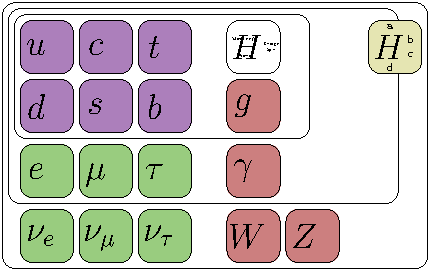
\includegraphics[scale=1.6]{texfig/SM}
\captionsetup{width=.8\linewidth}
\caption{A schematic of the Standard Model.}
\label{fig:sm}
\end{figure}

This analysis revolves around decays of the so-called $B$ mesons, which are particles that consist of a $b$ quark and a light $\bar u$ or $\bar d$ quark (or vice-versa). One of the most surprising features of the universe that can be studied with decays of $B$ mesons is the $CP$ symmetry violation ($\cancel{CP}$). $CP$ symmetry is a combination of the $C$ symmetry (charge conjugation) and the $P$ symmetry (spatial inversion). It states that there is no reason why processes of particles and mirrored processes of antiparticles would be different. Today we know that this does not hold for all cases and we, in fact, find processes which violate this postulate. We also know that $\cancel{CP}$ is very closely related to the weak nuclear force. Here lies our motivation for studying decays of $B$ mesons, since they exhibit a rich spectrum of decays, many of which underway via the weak nuclear force.

One of the most important properties of the weak nuclear force is that it can change the flavor of particles. Flavor is a quantum number which is conserved for each type of quark, so changing a flavor of a quark means changing the quark itself. Such processes are forbidden for the electromagnetic and the strong nuclear force, but not for the weak one. All of the information regarding quark transitions and transition probabilities can be merged into a form of a complex matrix called the Cabibbo-Kobayashi-Maskawa (CKM) matrix \cite{cabibbo1963unitary,kobayashi1973cp}
\begin{equation}
V_{CKM} = \begin{bmatrix}
    V_{ud} & V_{us} & V_{ub}\\
    V_{cd} & V_{cs} & V_{cb}\\
    V_{td} & V_{ts} & V_{tb}
\end{bmatrix}.
\end{equation}

The CKM matrix is a unitary matrix and has only four free parameters which are not described by theory. Its unitarity provides us with several mathematical identities, out of which the most famous one is
\begin{equation}
V_{ud}V_{ub}^* + V_{cd}V_{cb}^* + V_{td}V_{tb}^* = 0.
\end{equation}

It can be represented by a triangle in the complex plane, called the unitarity triangle, shown in Figure~\ref{ut}. The sides and the angles of the unitarity triangle are closely connected to the free parameters of the CKM matrix. It is important to mention that all experimental measurements depend only on these four parameters, so it is possible to determine them by measuring the angles and sides of the unitarity triangle. This way the unitarity triangle offers us a unique way to test the consistency of the SM. The ultimate goal is to then join all such measurements and overconstrain the unitarity triangle to check if all the sides meet. By improving such measurements one can check whether the SM is consistent, or if there are some contributing physics processes that we do not yet understand. Such processes are commonly referred to as "new physics" (NP). The measurements of the sides and angles of the triangle are done by using different decays of which a large portion are $B$ meson decays. Here lies another motivation for using $B$ mesons in the analysis.

\begin{figure}[H]
\centering
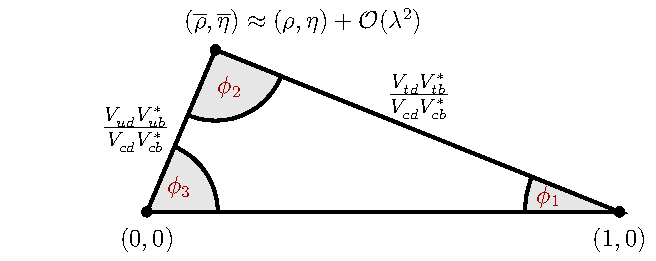
\includegraphics[scale=1]{texfig/UT_Triangle}
\caption{The unitarity triangle with $\lambda,~\eta,~\rho$ and $A$ (not shown) as free parameters of the CKM matrix.}
\label{ut}
\end{figure}

In this analysis, we focus on the $V_{ub}$ CKM matrix element, which corresponds to $b \to u$ quark transitions. It has the smallest absolute value of all the CKM matrix elements and the largest error, so it offers the most room for improvement. Such quark transitions are present in charmless semi-leptonic $B$ meson decays of the form
\begin{equation}
B^+ \to X_u^0 \ell^+ \nu_\ell,
\end{equation}

where $X_u^0$ represents a charmless hadron with a $u$ quark and $\ell$ is one of the charged leptons $e,~\mu$ or $\tau$. Measuring the decay rate of the $B$ meson in such decays paves the way for the CKM matrix element determination. Decay rates are directly connected to the $V_{ub}$ element as
\begin{equation}
\mathrm{d} \Gamma \propto G_F^2 \vert V_{ub} \vert ^2 \vert L^\mu \langle X_u \vert \bar u \gamma_u \frac{1}{2} (1-\gamma_5) b \vert B \rangle \vert ^2,
\end{equation}

where $\Gamma$ is the decay width, $G_F$ is the Fermi coupling constant, $L^\mu$ is the leptonic current and the expression in the Dirac brackets is the hadronic current. The factor $\vert V_{ub} \vert ^2$ represents the probability for the $b \to u$ quark transition. Measurement of the $V_{ub}$ CKM matrix element can be performed in two possible ways. With the exclusive or the inclusive method, which are described below. Both methods require different experimental and theoretical techniques, so they provide largely independent determinations of $\vert V_{ub} \vert$. Currently, both methods also have comparable accuracies. 

In the exclusive method, one studies the decays of $B$ mesons to a specific charmless hadronic final state, such as $B \to \pi \ell \nu$. Clean determination of the $V_{ub}$ is possible due to precise experimental measurements along with reliable theoretical calculations. However, theoretical calculations are more challenging for decays to a specific final state, since hadronization of quarks has to be taken into account. There are also two main experimental challenges in this method. One has to reduce the abundant background from $B \to X_c \ell \nu$ processes since the $b \to c$ quark transition is much more common. The second experimental challenge is to separate the $B$ meson decay with the specific charmless hadronic final state from other $B \to X_u \ell \nu$ decays since it roughly populates the same regions of the phase-space as the signal decay.

In the inclusive method, one studies the decays of $B$ mesons to any charmless hadronic final state $B \to X_u \ell \nu$. In this case, the total decay rate for $b \to u \ell \nu$ can be calculated accurately since hadronization does not have to be taken into account. The greater challenge with this method is again the experimental measurement of the total decay rate due to the $B \to X_c \ell \nu$ background. Experimental sensitivity to $V_{ub}$ is highest where $B \to X_c \ell \nu$ decays are less dominant. Theory and experiment have to compromise and limit the $V_{ub}$ determination to a region where the signal-to-background ratio is good. Theory takes this into account by reliably calculating the partial decay rate $\Delta \Gamma$, which is more challenging than the total decay rate. One possible and often used approach to reduce $b \to c$ background is to reject all events with $K$ particles, or kaons, present in the final particle selection. The procedure is called a $K$-veto. Kaons consist of an $s$ quark, which is mainly produced in $c \to s$ transitions. This means that if a kaon is found in the event, it is very likely that it originates from a particle with a $c$ quark, indicating the $b \to c$ process. 

If $V_{ub}$ is determined with both these methods, the values can be compared. It turns out that consistency between these two results is only marginal, where the difference is at a level of $3\sigma$. The current world averages \cite{Amhis:2016xyh} of the exclusive (from $B^0 \to \pi^- \ell^+ \nu$) and inclusive (GGOU collab. \cite{Gambino:2007rp}) are
\begin{align}
&\vert V_{ub} \vert_{\mathrm{excl.}} = \left(3.65 \pm 0.09 \pm 0.11\right)\E{-3},\\
&\vert V_{ub} \vert_{\mathrm{incl.}}^{\mathrm{GGOU}} = \left(4.52 \pm 0.15~{}^{+0.11}_{-0.14}\right)\E{-3},
\end{align}
where the first and the second errors are the experimental and the theoretical error, respectively. We see that inclusive measurements prefer higher values than exclusive ones. This is known as the $V_{ub}$ puzzle. It is necessary to make further research as to why this difference occurs. The reason could be an unknown experimental or theoretical error, or it is even possible that some NP contributions occur. This analysis will focus on a possible reason that could be hidden in the selection mentioned before. By performing a $K$-veto, one discards all events with kaons in the final state in order to suppress $b \to c$ contributions. In this analysis, we focus on the charged \decaya~decay, which is very similar to the $B \to \pi \ell \nu$, except for a production of an $s \bar s$ quark pair, which then combines with final state quarks to form kaons, as shown in Figure~\ref{feynman}. In this case, we have kaons in the final state where the $B$ meson decayed via a $b \to u$ process. Such decays were discarded in previous $V_{ub}$ determinations with the inclusive method, but in principle, they contribute to the result and should be taken into account. The results of this analysis should help us make a step closer to solving the $V_{ub}$ puzzle. 

\begin{figure}[H]
\centering
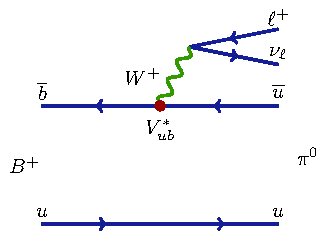
\includegraphics{texfig/B2pilnu}
\hspace{1cm}
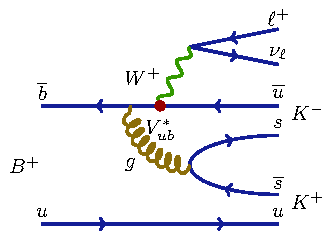
\includegraphics{texfig/B2KKlnu}
\caption{Feynman diagrams for the $B^+ \to \pi^0 \ell^+ \nu_\ell$ decay (left) and the $B^+ \to K^- K^+ \ell^+ \nu_\ell$ decay (right).}
\label{feynman}
\end{figure}

Specifically, we will be focusing on decays of the charged $B$ mesons of the form \decayb, since it includes two charged kaons, as opposed to the case of the neutral $B$ meson decay. The reason for this is a simpler decay chain and a higher reconstruction efficiency. All further occurrences of \decaya~automatically imply decays of the form \decayb~and its charge conjugated counterpart.